\documentclass[a4paper,14pt]{article}
\usepackage{extsizes}
\usepackage{amsmath}
\usepackage{amssymb}
\everymath{\displaystyle}
\usepackage{geometry}
\usepackage{fancyhdr}
\usepackage{multicol}
\usepackage{graphicx}
\usepackage[brazil]{babel}
\usepackage[shortlabels]{enumitem}
\usepackage{cancel}
\columnsep=2cm
\hoffset=0cm
\textwidth=8cm
\setlength{\columnseprule}{.1pt}
\setlength{\columnsep}{2cm}
\renewcommand{\headrulewidth}{0pt}
\geometry{top=1in, bottom=1in, left=0.7in, right=0.5in}

\pagestyle{fancy}
\fancyhf{}
\fancyfoot[C]{\thepage}

\begin{document}
	
	\noindent\textbf{7FMA154, 7FMA155~-~Matemática} 
	
	\begin{center}Inclinação de uma reta no plano (Versão estudante)
	\end{center}
	
	
	\noindent\textbf{Nome:} \underline{\hspace{10cm}}
    \noindent\textbf{Data:} \underline{\hspace{4cm}}
	
	%\section*{Questões de Matemática}
	
	\begin{multicols}{2}
		Observe os triângulos T1, T2 e T3 e responda as questões 1 e 2.
		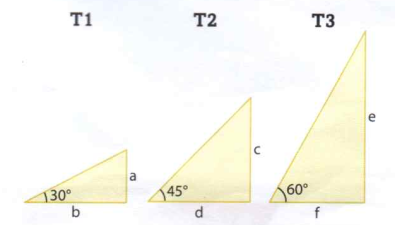
\includegraphics[width=0.45\textwidth]{/home/hogdelta/Documentos/latex/7FMA154_imagens/pg67.png}
	    \begin{enumerate}
	    	\item Se você ampliar ou reduzir os triângulos, as medidas dos lados mudarão, mas os ângulos não. As inclinações das hipóteses irão mudar ou não? Explique sua resposta.
	    	\\\\\\\\\\\\
	        
	    	\item Complete a tabela a seguir, estabelecendo a correspondência da inclinação como medida do ângulo e a inclinação como uma razão (representada por m). \\\\
		    
		    \begin{center}	
		    	% Início da tabela
		    	
		    	\begin{tabular}{|c|c|} % Define cinco colunas centradas com linhas verticais
		    		\hline % Linha horizontal no topo da tabela
		    		\textbf{Ângulo} & \textbf{\textit{m}} \\ % Conteúdo da primeira linha da tabela
		    		\hline % Linha horizontal
		    		30° & ~~~~~~~~~~~~ \\ % Conteúdo da segunda linha da tabela
		    		\hline % Linha horizontal
		    		45° & ~~~~~~~~~~~~ \\ % Conteúdo da terceira linha da tabela
		    		\hline % Linha horizontal no final da tabela
		    		60° & ~~~~~~~~~~~~ \\ % Conteúdo da terceira linha da tabela
		    		\hline % Linha horizontal no final da tabela
		    	\end{tabular}
	    	\end{center}
	    	\item Com base em seus conhecimentos sobre triângulos, mostre como podemos obter os valores de m do exercício 2.
	    	\\\\\\\\\\\\
	    	\item No gráfico a seguir, dê a inclinação das retas r, s, t e u:
	    	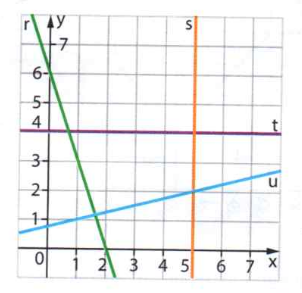
\includegraphics[width=0.45\textwidth]{/home/hogdelta/Documentos/latex/7FMA154_imagens/pg71.png}
	    	\item Em um plano cartesiano, apresente três retas e determine suas inclinações.\\\\\\\\\\\\
	    	\item 
	    	\begin{enumerate}[a)]
	    		\item Usando a racionalização de denominadores mostre que $\frac{1}{\sqrt{3}} = \frac{\sqrt{3}}{3}$\\\\\\\\\\\\\\
	    		\item O que podemos concluir sobre o produto dos valores de m para os ângulos de 30° e 60°?\\\\\\\\\\
	    		\item Sendo $\alpha$ e $\beta$ ângulos agudos de um triângulo retângulo, mostre que os valores de $m$ para $\alpha$ e $\beta$ tem produto igual a um.\\\\
	    	\end{enumerate}
    	    \item Usando a figura a seguir, calcule o valor de $m$ para o ângulo de 58°.\\
    	    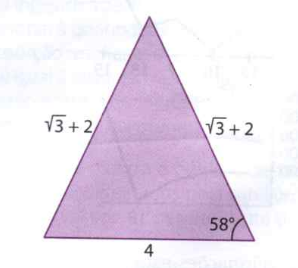
\includegraphics[width=0.45\textwidth]{/home/hogdelta/Documentos/latex/7FMA154_imagens/pg85-1.png} \\\\\\\\
    	    \item Sejam $r$ e $s$ as retas das equações $3x + 8y = 24$ e $y = 2x - 4$, respectivamente.
    	    \begin{enumerate}[a)]
    	    	\item No plano cartesiano da figura a seguir, trace as retas $r$ e $s$ e indique suas interseções com os eixos coordenados.\\
    	    	\noindent
    	    	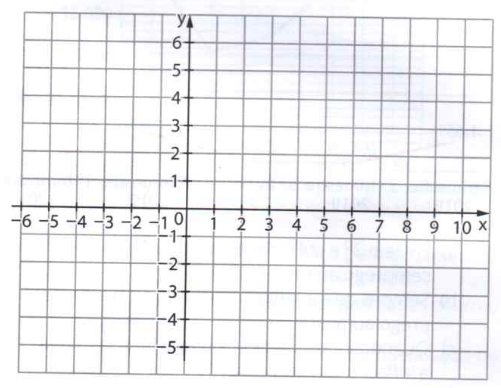
\includegraphics[width=0.35\textwidth]{/home/hogdelta/Documentos/latex/7FMA154_imagens/pg85-2.png}
    	    	\item Calcule a inclinação das retas $r$ e $s$.\\\\\\\\
    	    \end{enumerate}
        	\item Em relação ao exercício anterior, escreva uma equação da reta $r$ na forma $y = ax + b$. O que podemos concluir sobre $a$ para as duas retas, $r$ e $s$?
   	    \end{enumerate}
    \end{multicols}
\end{document}









